\documentclass[11pt]{article}
\usepackage[margin=1in]{geometry}
\usepackage{amsmath,amssymb,amsthm}
\usepackage{booktabs}
\usepackage{array}
\newcolumntype{L}[1]{>{\raggedright\arraybackslash}p{#1}}
\usepackage{graphicx}
\usepackage{xcolor}
\usepackage{microtype}
\usepackage[colorlinks=true,linkcolor=blue!50!black,citecolor=blue!50!black,urlcolor=blue!50!black]{hyperref}
\newtheorem{theorem}{Theorem}[section]
\newtheorem{proposition}[theorem]{Proposition}
\newtheorem{lemma}[theorem]{Lemma}
\newtheorem{corollary}[theorem]{Corollary}
\theoremstyle{definition}
\newtheorem{definition}[theorem]{Definition}
\newtheorem{computation}[theorem]{Computation}
\newtheorem{conjecture}[theorem]{Conjecture}
\newtheorem{crossing}{Crossing}
\theoremstyle{remark}
\newtheorem{remark}[theorem]{Remark}
\newcommand{\R}{\mathbb R}
\newcommand{\C}{\mathbb C}
\newcommand{\Z}{\mathbb Z}
\newcommand{\F}{\mathbb F}
\newcommand{\PA}{\mathrm{PA}}
\newcommand{\ZFC}{\mathrm{ZFC}}
\newcommand{\Con}{\mathrm{Con}}
\newcommand{\Tst}{T^{*}}
\newcommand{\PS}{\mathcal P}
\newcommand{\Hrec}{H_{\mathrm{record}}}
\newcommand{\Ree}{\operatorname{Re}}
\newcommand{\tr}{\operatorname{tr}}
\title{Arithmophysics\\ \large Geometry, quantum theory, the primes, and the border,\\ with the identities that cross them}
\author{Christophe Michaels}
\date{October 5, 2026}
\begin{document}
\maketitle

\begin{abstract}
\noindent \emph{Arithmophysics} is the name the author gave, in the first compilation of this programme, to the study of the primes through the objects of physics: oscillation, spectrum, confinement. That compilation carried an uncertainty-principle argument that was later corrected (theory atlas, entries P16--P18). This paper is the return to the name with the mathematics that was built in between. It has four chapters, one for each strand the programme now has, and each chapter states only what is proved or computed in that strand: the geometry (the explicit formula as a sum of oscillators, the light cone, the horn, the fold, the curve), the quantum theory (the two Hamiltonians that exist, the Möbius state, the inner product that does not yet exist), the primes (the running proof's target and what has been proved around it), and the border (the Gödel theorem, the potential set, the conjecture). The fifth chapter is the point of the paper: seven crossings, each an exact identity or a proved equivalence between two strands, with its proof or citation, ending at the single object none of the four strands supplies. Every physical word in this paper names a theorem, a computation, or a labelled conjecture. Nothing here proves the Riemann Hypothesis.
\end{abstract}

\tableofcontents

\section*{Status conventions and the rule of the word}
A \textbf{Theorem}, \textbf{Proposition} or \textbf{Lemma} without a citation is proved here or in the cited document of the programme, where the proof is complete; with a citation to the literature it is taken from there with its hypotheses. A \textbf{Computation} carries its file in the repository. A \textbf{Crossing} is an identity or a proved equivalence joining two strands. A \textbf{Conjecture} is labelled and never used.

The rule of the word: in this paper ``oscillator'', ``Hamiltonian'', ``horizon'', ``light cone'', ``trace'', ``inner product'', ``witness'' each name a specific mathematical object defined where the word first appears. The physics is a dictionary, not an argument. Where the early compilation used the physics as an argument (the error-fluctuation uncertainty principle), the atlas records the correction \cite[P17--P18]{atlas}, and nothing of that argument is used here.

\section{Geometry: the shape of the explicit formula}\label{sec:geo}

\subsection{The sum of oscillators}
For $f$ real with compact support, $g=f\star\tilde f$, $\hat g=|\hat f|^2$, Weil's explicit formula in the normalization of \cite{window} reads
\begin{equation}\label{eq:weil}
\sum_\rho\hat g\Big(\frac{\rho-\frac12}{i}\Big)=W_\infty(g)+\hat g(\tfrac i2)+\hat g(-\tfrac i2)-\sum_{n\ge2}\frac{\Lambda(n)}{\sqrt n}\big(g(\log n)+g(-\log n)\big).
\end{equation}
Read in $u=\log x$: the zero $\rho=\tfrac12+i\gamma$ contributes the oscillator $e^{i\gamma u}$ to the prime side, and the prime power $n$ contributes a point mass of weight $\Lambda(n)/\sqrt n$ at $u=\log n$ to the zero side. Each side is the spectrum of the other. In this paper ``oscillator'' means a term $e^{i\gamma u}$ of the left side of \eqref{eq:weil} and nothing else.

\subsection{The light cone}
For $f$ supported in $[-a,a]$ only the prime powers with $\log n<2a$ enter \eqref{eq:weil}. This is the cone of \cite[\S12]{folds}: half-width $a$ as time, $\log n$ as space, the edge $\log n=2a$, the entry of $n$ at $a_n=\tfrac12\log n$. The odd floor $\lambda(a)$ is the infimum of the form over odd unit $f$ supported in $[-a,a]$; it is attained and non-increasing \cite[Lemma 1.4]{window}.
\begin{theorem}[Weil \cite{weil52}; Yoshida \cite{yoshida}]\label{thm:weil}
$\mathrm{RH}\iff\lambda(a)\ge0$ for every $a>0$.
\end{theorem}
\begin{theorem}[Zhu {\cite[Thm.\ 6.2]{zhu}}]\label{thm:zhu}
$8.206\times10^{-15}\le\lambda(0.8)\le2.347\times10^{-14}$, certified; so $\lambda>0$ on $(0,0.8]$.
\end{theorem}
The horizon is $\Tst(a)=2\pi e^{2a}$: the height at which the Riemann--von Mangoldt density $(2\pi)^{-1}\log(t/2\pi)$ equals the Cartwright bound $a/\pi$ on the zero density of a function of exponential type $a$ \cite[\S1]{window}.
\begin{computation}[the floor; {\cite{folds,window}}]\label{comp:floor}
From \texttt{floor\_grid\_K40.csv} and \texttt{floor\_grid\_arb.csv}: $\lambda(0.3)=0.2226$, $\lambda(0.549)=1.49\times10^{-5}$, $\lambda(1.2)=7.2\times10^{-37}$, and $\lambda(1.505)\approx10^{-93}$ by certified enclosure. The floor is positive at every support computed; the horizon at $a=1.5$ is $\Tst=126$. Prime $2$ enters at $a=0.3466$ and is needed by $a=0.3716$.
\end{computation}

\subsection{The horn}
Draw the $n$-th zero as a circle of circumference $\gamma_n$ at height $n$ \cite[\S10]{folds}. Ring $n$ has radius $r_n=\gamma_n/2\pi$, and the surface of revolution has profile the inverse of the counting function: $n=r(\log r-1)+\tfrac78+S$, $S=O(\log\gamma_n)$.
\begin{computation}[{\cite{horn}}; \texttt{rh\_horn.py}, 6{,}000 zeros]\label{comp:horn}
Growth per ring $0.2239$ against $1/\log r=0.2238$ (first $1{,}000$ rings); rings minus law in $[-0.35,1.36]$; Riemann--Siegel phase advance $1.00003\,\pi$ per ring; $85.3$ percent of Gram intervals hold exactly one ring. The slope $1/\log r$ falls from $1.23$ at ring $1$ to $0.14$ at ring $6{,}000$: a horn, not a cone.
\end{computation}
The horn is hollow by construction, and only zeros on the line can be drawn as rings while the counting law counts every zero: for the Davenport--Heilbronn function the ring count drops by $2$ at each off-line pair \cite[Fig.\ 26C]{folds}.

\subsection{The fold}
The functional equation is the reflection $s\mapsto1-\bar s$, whose fixed set is the line $\Ree s=\tfrac12$ \cite[\S8]{folds}. The exponent dictionary \cite[Thm.\ 2.10]{horizon}: a bound $M(x)\ll x^{1/2+\theta+\varepsilon}$ confines every zero to the shell $|\Ree s-\tfrac12|\le\theta$, symmetric by the fold, hollow because the bound says nothing about the inside; what is known unconditionally is $\theta=\tfrac12-o(1)$, the whole strip less a sliver; the Hypothesis is that the shell has thickness zero.

\subsection{The curve}
For a curve $X/\F_q$ of genus $g$ with Frobenius eigenvalues $\alpha_i=\sqrt q\,e^{i\theta_i}$, the same construction gives the cone at support $D$ (closed points of degree $\le2D$ inside, half-width $a=D\log q$), the Toeplitz form $T_{2D+1}=[\hat\nu_X(j-k)]$ with $\hat\nu_X(m)=q^{m/2}+q^{-m/2}-N_mq^{-m/2}$, and the horn with rings at radii $(\theta_i/2\pi+k)/\log q$.
\begin{theorem}[{\cite[\S2]{ffcone}}]\label{thm:ffcone}
$T_{2D+1}$ is positive definite for $D<g$ and singular for $D\ge g$, with null vector the coefficients of $\prod_i(w-\bar z_i)$, $z_i=\alpha_i/\sqrt q$; the potential set is $\{\nu_X\}$ from $D=g$ on; the even sector closes at $D=g$, the odd at $g+1$; and $T_{2g+1}\succeq0$ if and only if every $|z_i|=1$. The horn of the curve is an exact cone of slope $1/(2g\log q)$, because the zeros are periodic in height.
\end{theorem}
The cone over a curve closes at $a=g\log q$; the cone over the integers never closes (Crossing~\ref{cr:edge}).

\section{Quantum theory: the operators}\label{sec:quantum}

\subsection{The stone-side Hamiltonian}
On $\ell^2(\mathbb N)=\bigotimes_p\ell^2(\mathbb N_0)$, with $S_pe_n=e_{pn}$ and $H_{\mathrm{arith}}e_n=(\log n)e_n$ \cite[\S2]{v32},
\[
[H_{\mathrm{arith}},S_p]=(\log p)S_p,\qquad\tr e^{-sH_{\mathrm{arith}}}=\zeta(s)\quad(\Ree s>1).
\]
This is Julia's primon gas and the Bost--Connes system \cite{bc}. Its eigenvalues are the positions of the stones on the prime line; its partition function is $\zeta$ where $\zeta$ has no zeros. ``Hamiltonian'' here means a self-adjoint operator whose eigenvalues are the positions of one side of \eqref{eq:weil}.

\subsection{The rule-side Hamiltonian}
On $L^2((0,\infty),dx)$ the dilation $(U_tf)(x)=e^{t/2}f(e^tx)$ is unitary \cite[Part VI]{running}, $U_t=e^{itH_{\mathrm{dil}}}$ with
\[
H_{\mathrm{dil}}=-i\Big(x\frac d{dx}+\frac12\Big)=\frac{xp+px}2,\qquad H_{\mathrm{dil}}\,x^{\rho-1}=-i\big(\rho-\tfrac12\big)x^{\rho-1}=\big[\gamma-i(\beta-\tfrac12)\big]x^{\rho-1}
\]
for $\rho=\beta+i\gamma$. This is the operator of Berry and Keating \cite{bk}; the mode of a zero has a real eigenvalue exactly when the zero is on the line; and the modes are not in $L^2$. The operator has continuous spectrum filling $\R$ and selects no zero \cite{es}. In the coordinate $u=\log x$, $(\mathcal Tf)(u)=e^{u/2}f(e^u)$ conjugates it to $-i\,d/du$: the oscillators of Section~\ref{sec:geo} are its generalized eigenfunctions. The early compilation's modes $e^{(\beta-1/2)u}e^{i\gamma u}$ \cite[P18]{atlas} are these.

\subsection{The Möbius state}
\begin{proposition}[{\cite[Prop.\ 3.2]{horizon}}]\label{prop:mstate}
Let $m(u)=e^{-u/2}M(e^u)=(\mathcal T\,M(x)/x)(u)$. Then (i) $I_M(e^U)=\int_0^U|m|^2$; (ii) $\int_0^\infty m(u)e^{-(s-1/2)u}du=1/(s\zeta(s))$ for $\Ree s>1$; (iii) $m\notin L^2(0,\infty)$, unconditionally.
\end{proposition}
The state whose power is the running proof's energy has spectrum $1/(s\zeta(s))$ on the line, resonances at the zeros, and infinite total power.

\subsection{The inner product}
\begin{theorem}[Connes \cite{connes99}]\label{thm:connes}
$\mathrm{RH}$ is equivalent to the positivity of the Weil distribution: to the existence of an inner product on the test functions in which \eqref{eq:weil} is the trace of the action of the idele class group, the zeros appearing as an absorption spectrum.
\end{theorem}
The floor $\lambda(a)$ is this positivity at support $a$. The operator whose self-adjointness in that inner product would put the zeros on the line is not constructed; the six constraints it must satisfy are \cite[\S4]{horizon}.

\subsection{The curve, where every piece exists}
\begin{theorem}[Weil \cite{weil48}; trace formula {\cite[Ch.\ VI]{milneEC}}]\label{thm:curve}
$N_m=1+q^m-\tr(F^m\mid H^1(X))$, $|\alpha_i|=\sqrt q$. With $U=F/\sqrt q$ and $H_X=-i\log U$, $N_m=1+q^m-q^{m/2}\tr e^{imH_X}$, and $\mathrm{RH}_X$ is the unitarity of $U$, supplied by the positivity of the Rosati involution (genus one: Hasse's $\deg(m-nF)=m^2-a_1mn+qn^2\ge0$) and the Hodge index theorem on $X\times X$.
\end{theorem}
Katz and Sarnak \cite{katzsarnak} proved the random-matrix statistics of the $\theta_i$ over families; for $\zeta$ the same statistics are Montgomery's theorem in its restricted range and Odlyzko's computation \cite{montgomery,odlyzko}.

\section{The primes: the record}\label{sec:primes}

\subsection{The target}
$M(x)=\sum_{n\le x}\mu(n)$, $I_M(N)=\int_1^NM(t)^2t^{-2}dt$. The running proof's single target is
\begin{equation}\tag{H}\label{eq:H}
I_M(X)\le C_\varepsilon X^\varepsilon\quad(X\ge2)\ \text{for every }\varepsilon>0 .
\end{equation}
\begin{theorem}[{\cite[\S11]{summary}}; Littlewood {\cite[\S14.25]{titchmarsh}}]\label{thm:closing}
\eqref{eq:H} $\iff\mathrm{RH}$. The forward direction is the Mellin step: \eqref{eq:H} gives absolute convergence of $\int_1^\infty M(x)x^{-s-1}dx$ on $\Ree s>\tfrac12$, hence holomorphy of $1/\zeta$ there, hence no zeros there, and the fold removes the other side.
\end{theorem}

\subsection{What is proved around it}
\begin{theorem}[{\cite[Part XVII]{running}}]\label{thm:lifetime}
$I_M(N)=\sum_{u\le N}w_u(1/u-1/\min(v_u,N))$ over the levels of $|M|$, and $\mathcal E_\star(N)\le I_M(N)\le2\log N+\mathcal E_\star(N)$.
\end{theorem}
\begin{theorem}[{\cite[Thm.\ 3.1, \S4, \S7]{hrec}}]\label{thm:hrec}
$\Hrec\iff\mathrm{RH}$. The debit identity $\Delta_N=E(u_0)+2M(m)h(u_0)+E(W)-2\langle a,W\rangle$ is exact; its two positive terms are each $\ge(1-o(1))\,m/(24\log^2m)$; the signed cross term carries the cancellation; the cofactor-flow identity $E(x-U_px)=(1+\tfrac1p)R(L)-\tfrac2p M(L)m_1(L)$ holds with $|m_1|\le1$.
\end{theorem}
\begin{theorem}[{\cite{census}}, checked in \cite{censusaudit}]\label{thm:census}
Every target of the lifetime census is equivalent to $\mathrm{RH}$; every proved credit is below the allowance $N^{1/2+\varepsilon}$; the paid insertion range is the Legendre range $2^{\pi(Y)}\le\sqrt N$, beyond which the alternating cofactor sum meets the parity obstruction.
\end{theorem}
\begin{theorem}[{\cite{v32}}]\label{thm:v32}
For $a>1$ the Möbius coefficient state $m_a=\sum\mu(d)d^{-a/2}e_d$ has $\|m_a\|^2=\zeta(a)/\zeta(2a)$; a global bilateral all-prime unitary exists; the cumulative synthesis map is unbounded; its Euler update is $q_\alpha((I-r_pS_p)c)=(1+r_p^2)q_\alpha(c)-2r_p\Ree\langle W_\alpha c,D_pW_\alpha c\rangle$; the shell-ledger gate along a determining sequence is equivalent to $\mathrm{RH}$.
\end{theorem}
Every quantity proved in this strand is one the target already tolerates; the subpower exponent is the only non-finitary object in it, and it sits at infinity.

\section{The border: the logic}\label{sec:border}

\begin{theorem}[{\cite[Thms.\ 4.1, 5.1, 6.1]{gstring}}; \cite{dmr}]\label{thm:godel}
$\mathrm{RH}$ is $\ZFC$-equivalent to a $\Pi^0_1$ sentence $\rho$. Adding every true $\Sigma^0_1$ sentence to any theory containing Robinson arithmetic adds no theorem. $\PA\vdash\rho\leftrightarrow\Con(\mathrm Q+\rho)$ and $\ZFC\vdash\rho\leftrightarrow\Con(\PA+\rho)$. A refutation of $\rho$ has a witness provable in $\mathrm Q$; non-refutability implies truth. Any true principle establishing $\rho$ over $\PA$ is unprovable in $\PA$, not equivalent to a $\Sigma^0_1$ sentence, and proves $\Con(\mathrm Q+\rho)$.
\end{theorem}
\begin{proposition}[{\cite[Props.\ 2.2--2.3]{potential}}; {\cite[Prop.\ 2.11]{horizon}}]\label{prop:potential}
The potential set $\PS(a)$ of configurations the primes inside the cone cannot distinguish from the zeros is non-increasing, nonempty iff the form is nonnegative at support $a$, and $\bigcap_a\PS(a)=\{\nu_\zeta\}$ iff $\mathrm{RH}$. Under $\mathrm{RH}$ the form has no null vector at any finite support: the collapse happens only at $a=\infty$.
\end{proposition}
On a curve the pattern has a last stone (degree $2g$), $\mathrm{RH}_X$ for one curve is a finite check, and the positivity that closes it, Weil's, is a theorem; the Gödel constraints bite only where the pattern has no last stone. \emph{The Grammar of Things} \cite{grammar} says the same in the language of a circle of stones: the records and the rule are one object described twice, and the distance between them is a border, not a distance that accumulation crosses.
\begin{conjecture}[Michaels; {\cite[\S10]{gstring}}]\label{conj}
$\rho$ is not provable in $\ZFC$. If so, $\mathrm{RH}$ is true, every instance is provable, $\rho$ is independent, and the inner product of Section~\ref{sec:quantum} is a new universal axiom.
\end{conjecture}
Labelled a conjecture; used nowhere.

\section{The crossings}\label{sec:cross}

Each crossing joins two strands by an identity or a proved equivalence. The proofs are one line or a citation; the point is that they are exact.

\begin{crossing}[geometry $\times$ primes: the stones sit in the horn]\label{cr:horizon}
The prime power $m$ enters the cone at $a_m=\tfrac12\log m$, where $\Tst(a_m)=2\pi m$: in the horn's unit, ring radius $m$. The stone $m$ sits on the horn's axis at radius $m$ and has resolved $N(2\pi m)=m(\log m-1)+\tfrac78+O(\log m)$ rings.
\end{crossing}
\begin{proof}
$\Tst(a_m)=2\pi e^{\log m}=2\pi m$ and $r=T/2\pi$. The count is the Riemann--von Mangoldt law at $T=2\pi m$. Computed for every prime power to $1{,}000$ in \texttt{data/horn\_stones.json}: $2\mapsto0$ (the horizon $4\pi$ is below the first zero), $3\mapsto1$, $7\mapsto8$, $11\mapsto16$, $97\mapsto348$, $997\mapsto5{,}888$.
\end{proof}

\begin{crossing}[geometry $\times$ quantum: rings are wavenumbers]\label{cr:rings}
The ring of the zero $\gamma$ has radius $\gamma/2\pi$, the number of oscillations per $e$-fold of $x$ of the oscillator $e^{i\gamma\log x}$; the horn's slope $1/\log r$ is the mean spacing of the zeros in that unit; the Riemann--Siegel phase advances by $\pi$ per ring.
\end{crossing}
\begin{proof}
The oscillator has period $2\pi/\gamma$ in $u=\log x$; $r=1/\text{period}$. The mean gap at height $T$ is $2\pi/\log(T/2\pi)$, which is $1/\log r$ in radius. $\theta(t)=\pi[r(\log r-1)-\tfrac18]+O(1/t)$ and $N=\theta/\pi+1+S$; Computation~\ref{comp:horn} measures $1.00003\,\pi$.
\end{proof}

\begin{crossing}[quantum $\times$ primes: the target is a spectral statement]\label{cr:state}
\eqref{eq:H} holds iff the Möbius state has subexponential accumulated power, $\int_0^U|m|^2\le C_\varepsilon e^{\varepsilon U}$; its transform is $1/(s\zeta(s))$; $\mathrm{RH}$ is the statement that every resonance of the state has a real frequency.
\end{crossing}
\begin{proof}
Proposition~\ref{prop:mstate}(i)--(ii) and Theorem~\ref{thm:closing}.
\end{proof}

\begin{crossing}[geometry $\times$ quantum, on the curve: the cone closes when the matrix runs out]\label{cr:curve}
$N_m=1+q^m-q^{m/2}\tr e^{imH_X}$; the Toeplitz form of the cone at support $D$ is $\sum_i|\hat h(\theta_i)|^2$ over the $2g$ eigenphases; it acquires a null vector exactly when $2D+1>2g$, and the null vector's roots are the eigenphases. The horn of the curve is an exact cone because $H_X$ has finitely many eigenvalues, periodic in height.
\end{crossing}
\begin{proof}
Theorems~\ref{thm:curve} and \ref{thm:ffcone}; the genus-one case by hand in \cite{reading}: $N_1=6$, $N_2=12$, $a_1=-2$, the $3\times3$ form at $a=\log3$ with eigenvalues $0,\tfrac83,\tfrac{10}3$, null vector $(1,2/\sqrt3,1)$ with roots at $\cos\theta=-1/\sqrt3$.
\end{proof}

\begin{crossing}[primes $\times$ quantum: one signed cross term, in two normalizations]\label{cr:sign}
The Euler update of Theorem~\ref{thm:v32} and the cofactor-flow identity of Theorem~\ref{thm:hrec} have the same shape: a positive diagonal $(1+r_p^2)q$, respectively $(1+\tfrac1p)R$, and one signed cross term, $-2r_p\Ree\langle Wc,D_pWc\rangle$, respectively $-\tfrac2pM(L)m_1(L)$. In both, positivity fixes the total to be a square and leaves the sign of the cross term open; in both, that sign is the whole question, and in the census it is the parity obstruction.
\end{crossing}
\begin{proof}
Read the two identities side by side; the second is \cite[M44]{hrec}, the first \cite[\S3]{v32}. The parity statement is Theorem~\ref{thm:census}.
\end{proof}

\begin{crossing}[border $\times$ all: the edge, and what kind of thing each object is]\label{cr:edge}
The following are equivalent, each equivalence proved: $\mathrm{RH}$; \eqref{eq:H}; $\Hrec$; $\lambda(a)\ge0$ for all $a$; $\bigcap_a\PS(a)=\{\nu_\zeta\}$; the census residual bound; over $\ZFC$, $\Con(\PA+\rho)$. Under $\mathrm{RH}$ no finite support decides any of them. The inner product is a universal statement; a negative floor at one finite support, or one off-line zero, is a witness with a finite certificate.
\end{crossing}
\begin{proof}
\cite[Thm.\ 2.10, Prop.\ 2.11]{horizon}; the witness clause is Theorem~\ref{thm:godel} with Theorem~\ref{thm:weil}: $\lambda(a)<0$ is certifiable by interval arithmetic exactly as Theorem~\ref{thm:zhu} certifies $\lambda(0.8)>0$.
\end{proof}
\begin{remark}[the forced case]
The Davenport--Heilbronn function keeps the functional equation and drops the Euler product; its floor turns negative at a finite support, near $a\approx2.1$, where the horizon reaches its off-line zero at height $85.7$ \cite[Rem.\ 12.9]{folds}, and its horn loses two rings per pair. That is a witness for a cousin, and it says nothing about $\zeta$, which is the Euler-product filter of \cite{routes}. The same distinction appeared in fluid mechanics in September 2026, when a forced Navier--Stokes blow-up with bounded energy was announced while the unforced question stayed open \cite{ns}: a witness for a forced cousin, the conserved energy blind to it, the universal statement untouched. The parallel is in the logical type of the statements, not in the equations.
\end{remark}

\begin{crossing}[border $\times$ curve: where the pattern is finite the axiom is a theorem]\label{cr:finite}
On a curve the stones end at degree $2g$, the cone closes at $a=g\log q$, positivity at the single support $D=g$ is $\mathrm{RH}_X$, and Weil's positivity is a theorem of $\ZFC$. Over the integers the stones do not end, the cone does not close, no support decides, and any principle that closes it proves $\Con(\mathrm Q+\rho)$.
\end{crossing}
\begin{proof}
Theorems~\ref{thm:ffcone}, \ref{thm:curve}, \ref{thm:godel}; Proposition~\ref{prop:potential}.
\end{proof}

\subsection{The one object none of the strands supplies}
Geometry supplies the shape and shows where it closes. Quantum theory supplies two operators and names the third. The primes supply the record and locate its end at infinity. The border says what kind of statement the missing object's positivity must be. What none of them supplies is the inner product for $\zeta$: the space in which \eqref{eq:weil} is a trace, the positivity of which is the Hypothesis. Its specification is the six constraints of \cite[\S4]{horizon}: the trace with the prime sign handled, positivity equivalent to $\mathrm{RH}$, infinite genus with the growth of $N(T)$, entries as orbit half-lengths, the axiom-from-above form, and the function-field template. Deninger's foliated spaces \cite{deninger} and the arithmetic site of Connes and Consani \cite{cc16} are the candidates, each stalled at exactly the positivity. Arithmophysics, in the sense of this paper, is the study of that one missing object through the four that exist.

\section{Status}
\begin{center}\footnotesize
\begin{tabular}{L{0.54\textwidth}L{0.17\textwidth}L{0.2\textwidth}}
\toprule
statement & status & where\\
\midrule
explicit formula; Weil's criterion; Zhu's certified floor & cited & \S\ref{sec:geo}\\
cone, horizon, floor decay; horn, phase per ring, Gram's law & computed & Comp.~\ref{comp:floor}, \ref{comp:horn}\\
cone over a curve closes at $g\log q$; finite-support criterion & proved & Thm.~\ref{thm:ffcone}\\
two Hamiltonians; Berry--Keating identity; continuous spectrum & proved / cited & \S\ref{sec:quantum}\\
Möbius state: power, transform, infinite power & proved & Prop.~\ref{prop:mstate}\\
$\mathrm{RH}\iff$ positivity of the Weil distribution & cited & Thm.~\ref{thm:connes}\\
curve: trace formula, unitarity, Katz--Sarnak & cited & Thm.~\ref{thm:curve}\\
\eqref{eq:H} $\iff\mathrm{RH}$; lifetime truncation; $\Hrec$; census; Build v32 & proved / cited & \S\ref{sec:primes}\\
the subpower premise \eqref{eq:H} & \textbf{open} & \\
Gödel theorems; potential set; no null vector at finite $a$ & proved & \S\ref{sec:border}\\
Crossings 1--7 & proved & \S\ref{sec:cross}\\
the inner product for $\zeta$ & \textbf{not constructed} & \S\ref{sec:cross}\\
the Michaels Conjecture & conjecture & Conj.~\ref{conj}\\
the early uncertainty-principle argument & corrected, not used & \cite[P17--P18]{atlas}\\
the Riemann Hypothesis & \textbf{open} & \\
\bottomrule
\end{tabular}
\end{center}

\begin{center}
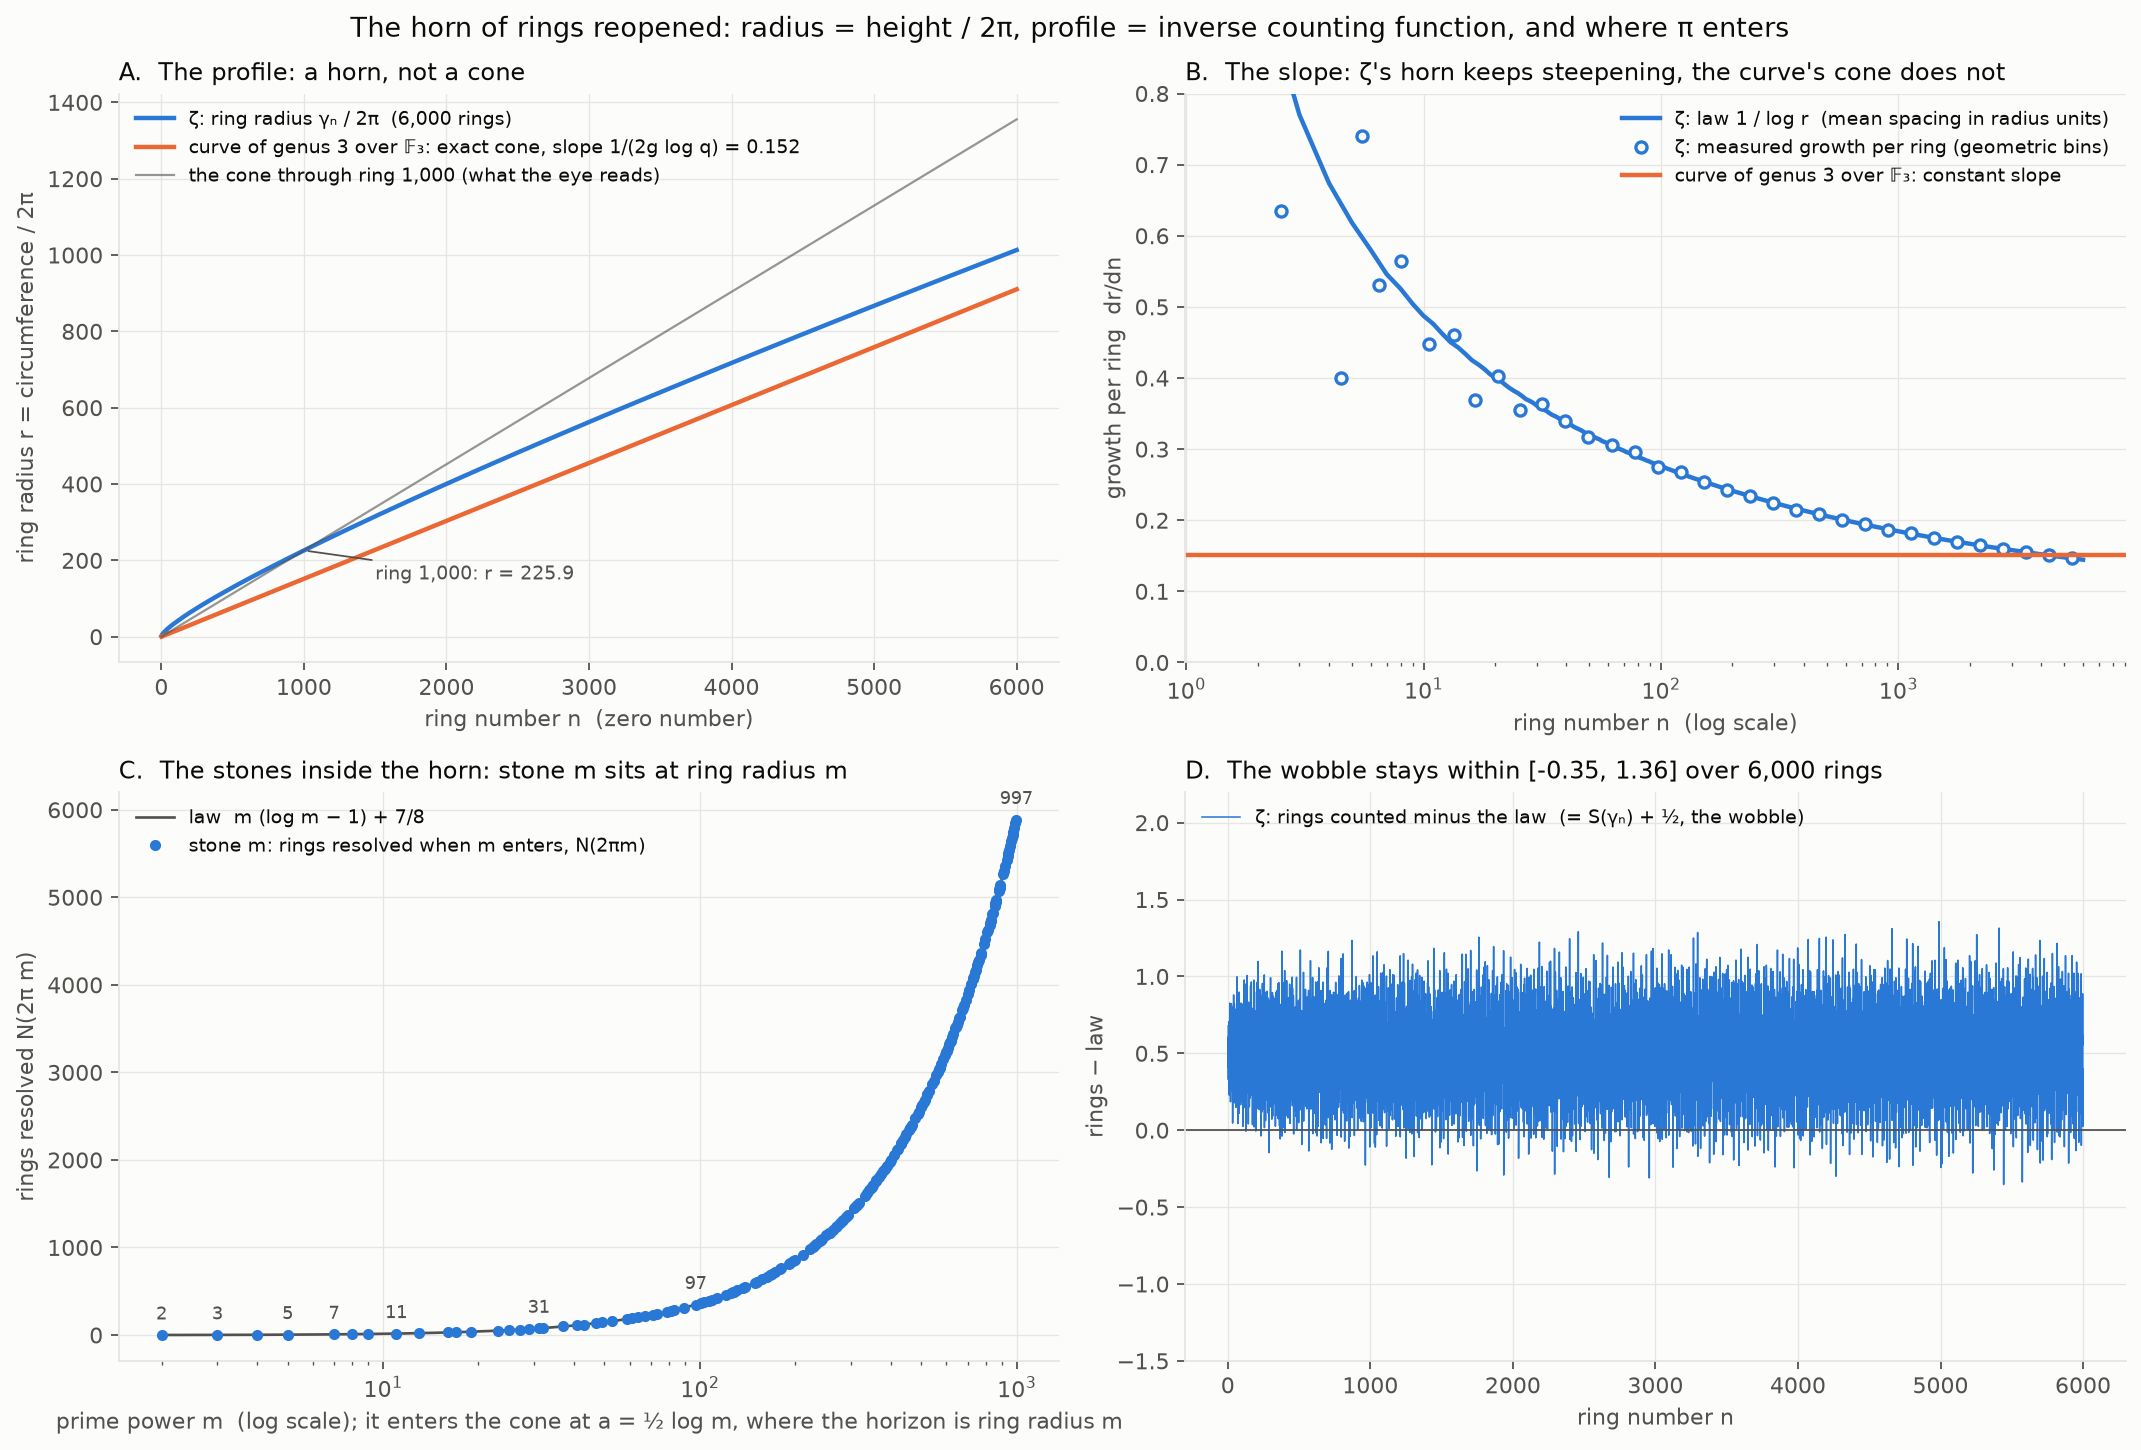
\includegraphics[width=\textwidth]{THE_HORN.png}
\end{center}
\noindent\emph{The horn: profile and slope against the exact cone of a curve, the stones inside at ring radius $m$, and the wobble} (\texttt{THE\_HORN.png}).
\begin{center}
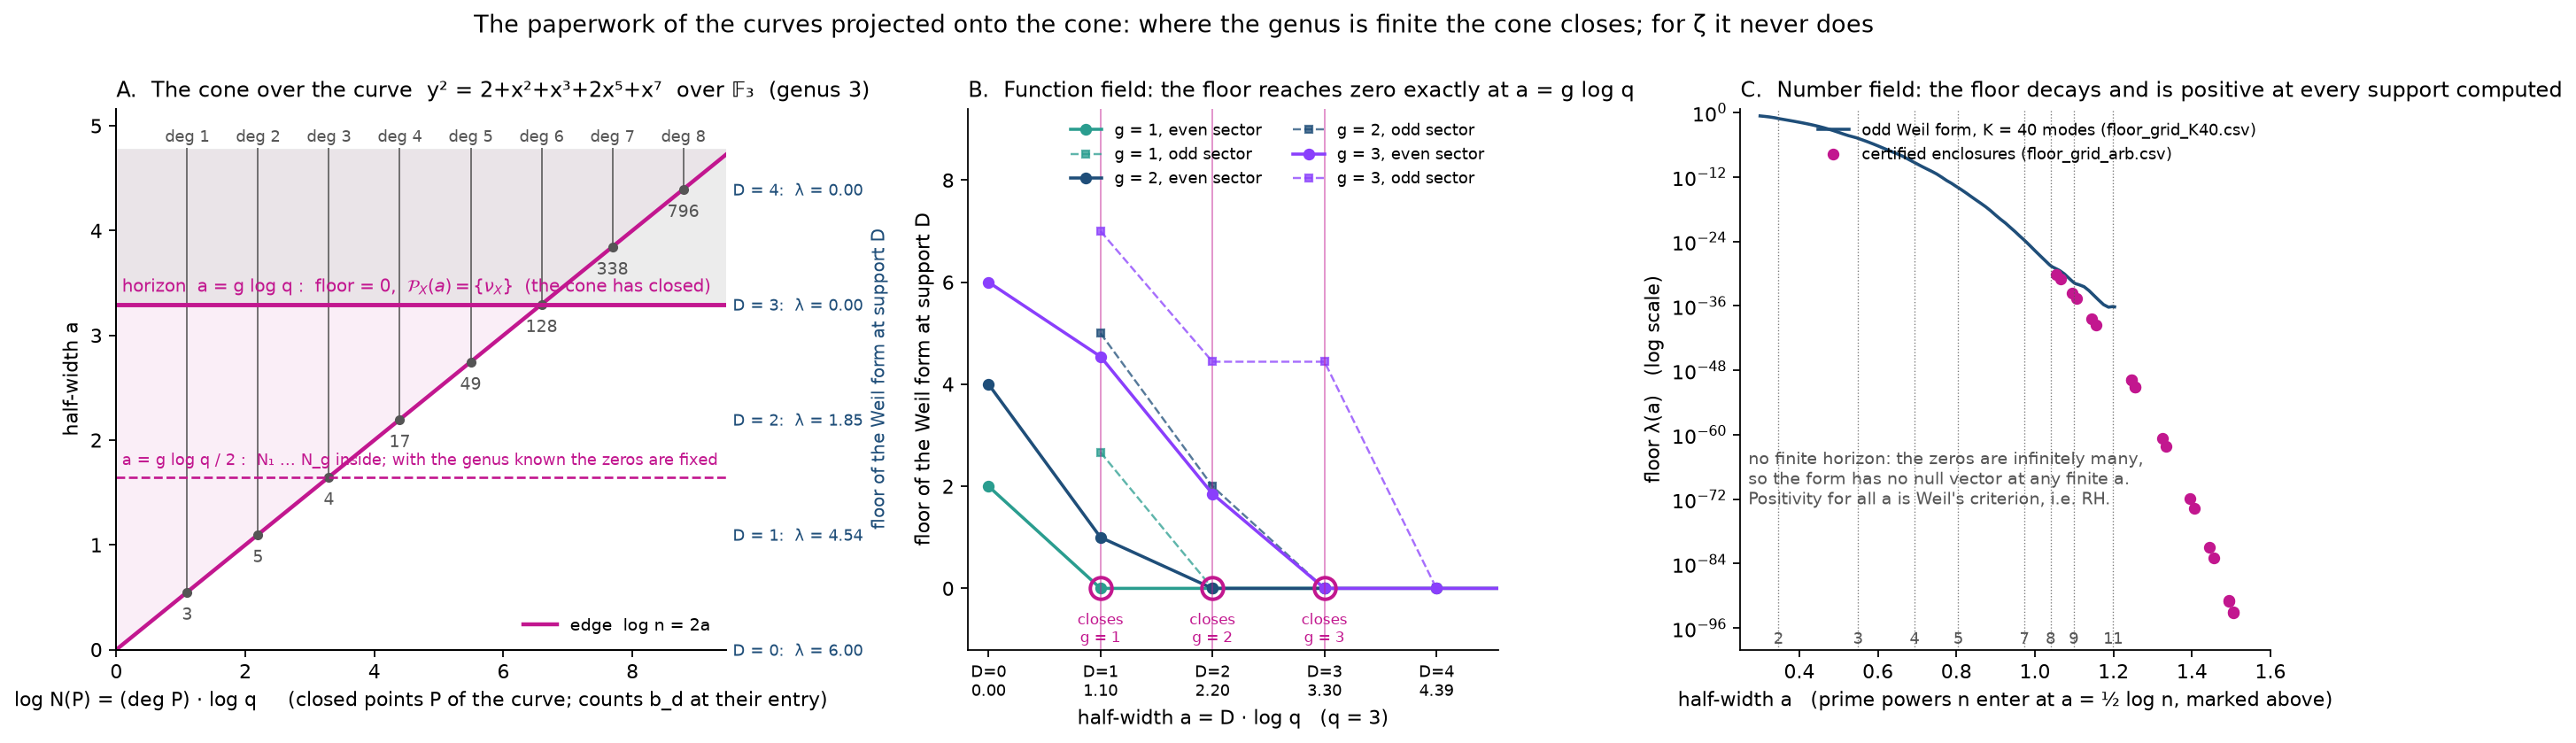
\includegraphics[width=\textwidth]{FUNCTION_FIELD_CONE.png}
\end{center}
\noindent\emph{The cone over a curve closing at $g\log q$; the number-field floor decaying and never reaching zero} (\texttt{FUNCTION\_FIELD\_CONE.png}).

\begin{thebibliography}{99}\small
\bibitem{atlas} C.~Michaels, \emph{Theta Kernels, Weil Positivity, and the Mathematical Theory Atlas}, through Checkpoint 20, September 23, 2026, atlas entries P16--P18 (\texttt{atlas/Michaels\_Theta\_Atlas\_CP20.pdf}, printed p.\ 482--483).
\bibitem{horizon} C.~Michaels, \emph{Across the Horizon}, \texttt{ACROSS\_THE\_HORIZON.pdf}, October 5, 2026.
\bibitem{running} C.~Michaels, \emph{Michaels Unified Running Proof}, Parts 0--XVII, October 4, 2026 (the opening 217 pages of the unified manuscript, master branch).
\bibitem{summary} C.~Michaels, \emph{Direct Historical-Energy Argument}, twelve-page companion, October 4, 2026.
\bibitem{hrec} C.~Michaels, \emph{The record estimate $\Hrec$}, \texttt{RESEARCH\_H\_RECORD.pdf}, October 3, 2026.
\bibitem{census} C.~Michaels, \emph{Lifetime Census and Closing Consequences}; \emph{The Complete Residual and a Fictional Closing Mechanism}, October 5, 2026, \texttt{received/}.
\bibitem{censusaudit} \texttt{RESEARCH\_CENSUS\_AUDIT.md}, October 5, 2026.
\bibitem{folds} C.~Michaels, \emph{Primes, Folds, and the One Dot}, draft of September 28, 2026, \texttt{received/Primes\_Folds\_One\_Dot\_paper.pdf}.
\bibitem{window} C.~Michaels, \emph{Prime DNA: The Floor of the Weil Form}, \texttt{weil\_window.pdf}, October 1, 2026.
\bibitem{potential} C.~Michaels, \emph{The potential set of the light cone}, \texttt{atlas\_potential\_set.pdf}, September 29, 2026.
\bibitem{gstring} C.~Michaels, \emph{RH on a G String}, \texttt{RH\_GODEL\_THEOREM.pdf}, October 5, 2026.
\bibitem{ffcone} \texttt{FUNCTION\_FIELD\_CONE.md}, October 5, 2026.
\bibitem{reading} \emph{Reading the curve}, \texttt{READING\_THE\_CURVE.pdf}, October 5, 2026.
\bibitem{horn} \emph{The horn of rings, reopened}, \texttt{THE\_HORN.md}, October 5, 2026.
\bibitem{v32} C.~Michaels, \emph{Prime DNA, Build v32: Prime-State All-Pass Geometry and the Observability Boundary}, August 25, 2026, \texttt{received/}.
\bibitem{routes} \texttt{RH\_ROUTES.md}, September 29, 2026.
\bibitem{grammar} C.~Michaels, \emph{The Grammar of Things}, July 2026.
\bibitem{weil52} A.~Weil, Sur les ``formules explicites'' de la th\'eorie des nombres premiers, \emph{Comm. S\'em. Math. Univ. Lund} (1952), 252--265.
\bibitem{yoshida} H.~Yoshida, On Hermitian forms attached to zeta functions, \emph{Adv. Stud. Pure Math.} 21 (1992), 281--325.
\bibitem{zhu} X.~Zhu, Weil positivity in compact windows, arXiv:2608.24827 (2026), Theorem 6.2.
\bibitem{bc} B.~Julia, Statistical theory of numbers, Springer Proc. Phys. 47 (1990); J.-B.~Bost and A.~Connes, \emph{Selecta Math.} 1 (1995), 411--457.
\bibitem{bk} M.~V.~Berry and J.~P.~Keating, $H=xp$ and the Riemann zeros (1999); \emph{SIAM Review} 41 (1999), 236--266.
\bibitem{es} S.~Endres and F.~Steiner, The Berry--Keating operator on $L^2(\mathbb R_>,dx)$, \emph{J. Phys. A} 43 (2010), 095204.
\bibitem{connes99} A.~Connes, Trace formula in noncommutative geometry and the zeros of the Riemann zeta function, \emph{Selecta Math.} 5 (1999), 29--106.
\bibitem{cc16} A.~Connes and C.~Consani, Geometry of the arithmetic site, \emph{Adv. Math.} 291 (2016), 274--329.
\bibitem{deninger} C.~Deninger, Some analogies between number theory and dynamical systems on foliated spaces, \emph{Doc. Math.} ICM I (1998), 163--186.
\bibitem{weil48} A.~Weil, \emph{Sur les courbes alg\'ebriques et les vari\'et\'es qui s'en d\'eduisent}, Hermann, 1948.
\bibitem{milneEC} J.~S.~Milne, \emph{Lectures on \'Etale Cohomology}, Ch.\ VI.
\bibitem{katzsarnak} N.~M.~Katz and P.~Sarnak, \emph{Random Matrices, Frobenius Eigenvalues, and Monodromy}, AMS, 1999.
\bibitem{montgomery} H.~L.~Montgomery, The pair correlation of zeros of the zeta function, \emph{Proc. Symp. Pure Math.} 24 (1973), 181--193.
\bibitem{odlyzko} A.~M.~Odlyzko, On the distribution of spacings between zeros of the zeta function, \emph{Math. Comp.} 48 (1987), 273--308.
\bibitem{titchmarsh} E.~C.~Titchmarsh, \emph{The Theory of the Riemann Zeta-Function}, 2nd ed., 1986, \S14.25.
\bibitem{dmr} M.~Davis, Y.~Matijasevi\v c and J.~Robinson, Hilbert's tenth problem, \emph{Proc. Symp. Pure Math.} 28 (1976), 323--378.
\bibitem{ns} K.~Kakaes, AI has solved one of math's \$1 million Millennium Prize problems, \emph{Quanta Magazine}, September 8, 2026; OpenAI, \emph{On the Navier--Stokes Millennium Prize Problem} (forced equations, bounded kinetic energy, unforced case not addressed).
\end{thebibliography}
\end{document}
